% -*- coding: utf-8 -*-
\documentclass{oblivoir}
\usepackage[utf8]{inputenc}
\usepackage{kotex}
\usepackage{graphicx}

\title{\textbf{넷마블 분석을 통한 효율적인 경영 방법 및 비젼 고찰}}
\author{\textbf{1학년 9반 15번 박태원}}

\begin{document}
	\maketitle
	\pagebreak
	
	\begin{center}
	\tableofcontents
	\pagebreak
	\end{center}

	\begin{abstract}
	
	\end{abstract}

	\section{서론}
		\subsection{배경 및 선정 동기}
			\textbf{게임 엔터테인먼트 산업}은 4차 산업혁명의 역풍에 굴하지 않고 꾸준히 각광받고 있는 산업이다. 이에 국내 시장에서는 2015년 최초로 \textbf{10조원}이상의 매출액을 기록한 이후, `16년에는 \textbf{11조원}, `17년에는 \textbf{12조원}, 가장 최근인 `18년에는 \textbf{13조원}을 기록하며 지속적인 성장세를 보여주고 있다.\footnote{콘텐츠산업 2018년 결산 및 2019년 전망 보고서 34p}
			
			\begin{figure}[htbp]
				\centering
				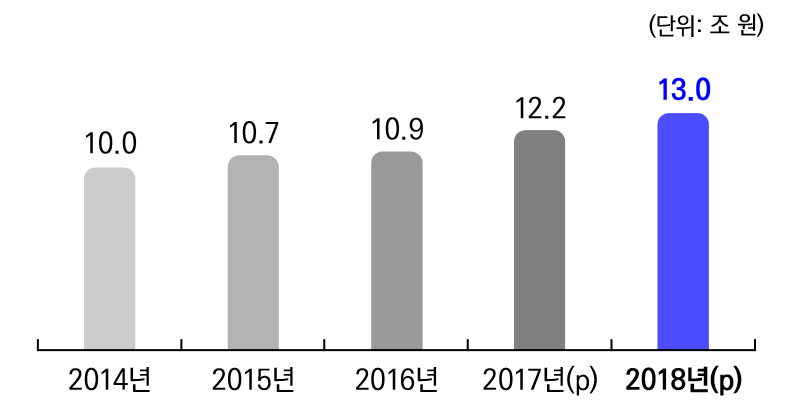
\includegraphics[width=1\textwidth]{GameMaechul.png}
				\caption{게임 산업 매출액 추이}
			\end{figure}
			
			또한 최근에는 \textbf{E-SPORTS 산업}의 성장으로 인해 \textbf{2020년까지 꾸준히 상승}할 것으로 전망되었다.\footnote{한국콘텐츠진흥원 대한민국 게임백서 2018 6p} 
			따라서 앞으로의 전망을 보았을 때, 게임 산업에 대해서 분석해볼 가치가 있다고 판단하였다.
			
			그 중에서도 넷마블은 국내에서 오랜 시간 명목을 이어오고 있는 게임 퍼블리셔 중 하나이며, 최근에는 리니지M 연 매출 2000억원을 달성하여 \textbf{"시장을 창조하였다"} 와 같은 평가를 받은 세계적인 게임 퍼블리셔로 성장하고 있다.
			이러한 관점에서 넷마블이 게임 산업을 연구하기에 적절한 기업이라 판단하였다.
			
			본 논문에서는 기업 분석과 연구를 기반으로 고찰하여 넷마블에 대한 \textbf{효율적인 경영 방법}과 \textbf{비젼}을 도출한다. 
			
		\subsection{절차}
			넷마블에 대한 분석은 다음과 같은 절차로 진행한다.
			
			\begin{description}
			\item[1. 시장 분석] - 시장의 환경이 기업에 끼치는 영향에 대하여 분석한다.
			\item[2. 환경 분석]
			\item[3. 경쟁사 분석]
			\item[4. 마케팅 분석]
			\item[5. 재무 분석]
			\item[6. 주가 분석] 
			\end{description}
	
	\section{선행 조사}
		\subsection{기업 개요}
		
		\subsection{기업 연혁}
		
		\subsection{기업 비전}
		
		\subsection{사업 분야}
	
	\section{본론}
		\subsection{방법}
		
		\subsection{시장 분석}
		
		\subsection{환경 분석}
		
		\subsection{경쟁사 분석}
		
		\subsection{마케팅 분석}
		
		\subsection{재무 분석}
		
		\subsection{주가 분석}
	
	\section{결론}
	
	\section{레퍼런스}
	

\end{document}